% 99-59(99쪽) — $\seg{AB}=5$ · $\seg{BC}=6$ 인 평행사변형 ABCD. 스캔 화질이 낮아 TikZ 로 다시 그림.
% 라벨은 원문 것만: 꼭짓점 A·B·C·D 와 길이 5·6. 각 $A$(답)는 그림에서 읽히지 않게 표시하지 않는다.
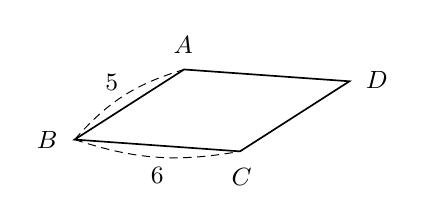
\begin{tikzpicture}[line width=0.6pt, x=1cm, y=1cm]
  \coordinate (A) at (1.39,0.89);
  \coordinate (B) at (0,0);
  \coordinate (C) at (2.10,-0.15);
  \coordinate (D) at (3.49,0.74);
  \draw (A) -- (B) -- (C) -- (D) -- cycle;
  % 길이 표시의 점선 호
  \draw[densely dashed, line width=0.35pt] (B) to[bend left=16] (A);
  \draw[densely dashed, line width=0.35pt] (B) to[bend right=14] (C);
  \node[font=\small, fill=white, inner sep=1pt] at (0.47,0.73) {$5$};
  \node[font=\small] at (1.05,-0.46) {$6$};
  \node[font=\small, anchor=south] at (1.38,0.96) {$\pt{A}$};
  \node[font=\small, anchor=east] at (-0.09,0.00) {$\pt{B}$};
  \node[font=\small, anchor=north] at (2.12,-0.24) {$\pt{C}$};
  \node[font=\small, anchor=west] at (3.57,0.76) {$\pt{D}$};
\end{tikzpicture}
